% ExVA/Lego/256:     u4108 -> lego_random_exr
%       150k:   24.00 & 0.88 & 0.101 & 0.207 & 150k & 256px & 11h30m
%       80k:    23.76 & 0.87 & 0.117 & 0.215 & 80k & 256px & 5h

\begingroup
\begin{figure}[!htb]
    % \setArraystrech{1.5}
    \centering
    \setlength\tabcolsep{2pt}
    \begin{tabular*}{\textwidth}{ c c c c c }
        HDRFlip$_{ExVA}$ & ExVA & Target & ExBF & HDRFlip$_{ExBF}$ \\
        % \multicolumn{2}{c}{256px} & 256px & \multicolumn{2}{c}{64px} \\
        256px & 256px & 256px & 64px & 64px \\
        
          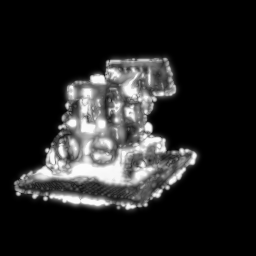
\includegraphics[width=0.19\textwidth]{figures/results/arb_set/validation/lego6_exva_hdrflip_150k.png}
        & 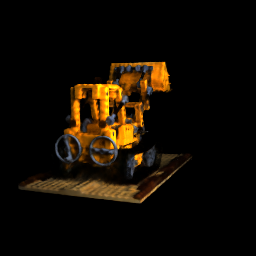
\includegraphics[width=0.19\textwidth]{figures/results/arb_set/validation/lego6_exva_150k.png}
        & 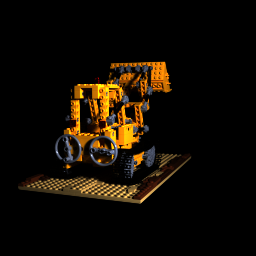
\includegraphics[width=0.19\textwidth]{figures/results/arb_set/validation/lego6_targ_256px.png}
        & 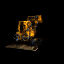
\includegraphics[width=0.19\textwidth]{figures/results/arb_set/validation/lego6_exbf_112k.png}
        & 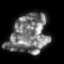
\includegraphics[width=0.19\textwidth]{figures/results/arb_set/validation/lego6_exbf_hdrflip_112k.png} \\[-6pt]
        
          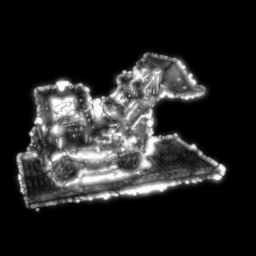
\includegraphics[width=0.19\textwidth]{figures/results/arb_set/validation/lego7_exva_hdrflip_150k.png}
        & 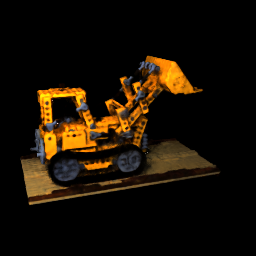
\includegraphics[width=0.19\textwidth]{figures/results/arb_set/validation/lego7_exva_150k.png}
        & 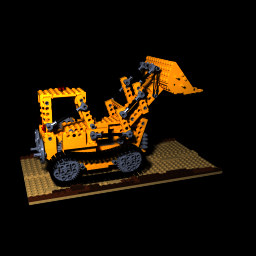
\includegraphics[width=0.19\textwidth]{figures/results/arb_set/validation/lego7_targ_256px.png}
        & 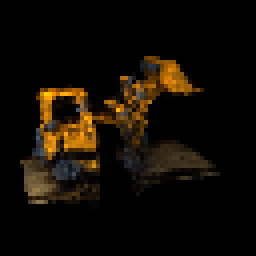
\includegraphics[width=0.19\textwidth]{figures/results/arb_set/validation/lego7_exbf_112k.png}
        & 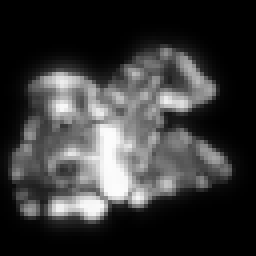
\includegraphics[width=0.19\textwidth]{figures/results/arb_set/validation/lego7_exbf_hdrflip_112k.png} \\[-6pt]
        
          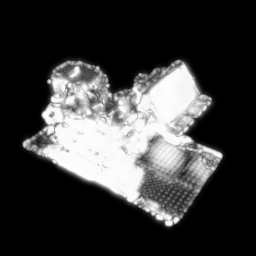
\includegraphics[width=0.19\textwidth]{figures/results/arb_set/validation/lego10_exva_hdrflip_150k.png}
        & 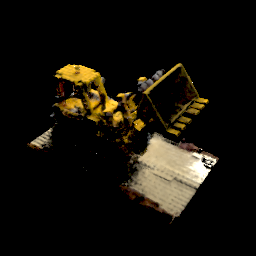
\includegraphics[width=0.19\textwidth]{figures/results/arb_set/validation/lego10_exva_150k.png}
        & 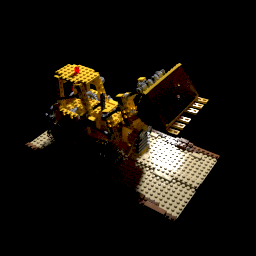
\includegraphics[width=0.19\textwidth]{figures/results/arb_set/validation/lego10_targ_256px.png}
        & 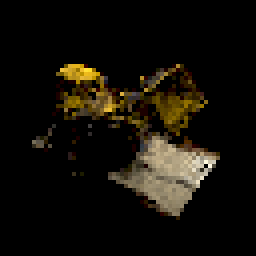
\includegraphics[width=0.19\textwidth]{figures/results/arb_set/validation/lego10_exbf_112k.png}
        & 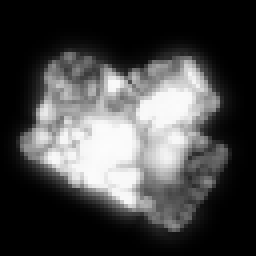
\includegraphics[width=0.19\textwidth]{figures/results/arb_set/validation/lego10_exbf_hdrflip_112k.png} \\[-6pt]
        
          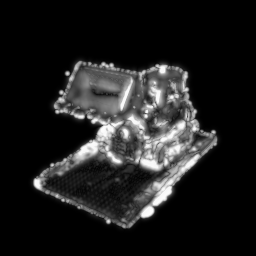
\includegraphics[width=0.19\textwidth]{figures/results/arb_set/validation/lego14_exva_hdrflip_150k.png}
        & 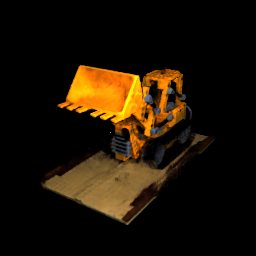
\includegraphics[width=0.19\textwidth]{figures/results/arb_set/validation/lego14_exva_150k.png}
        & 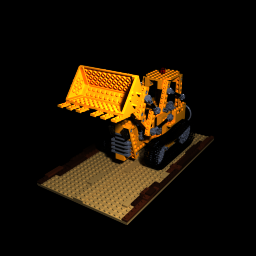
\includegraphics[width=0.19\textwidth]{figures/results/arb_set/validation/lego14_targ_256px.png}
        & 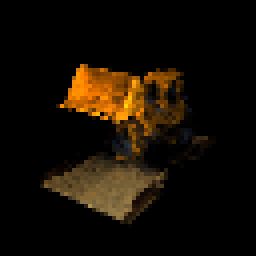
\includegraphics[width=0.19\textwidth]{figures/results/arb_set/validation/lego14_exbf_112k.png}
        & 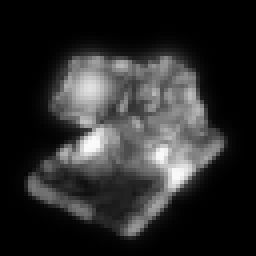
\includegraphics[width=0.19\textwidth]{figures/results/arb_set/validation/lego14_exbf_hdrflip_112k.png}
        

    \end{tabular*}
    \caption{The overview of some novel light-view synthesis results
    achieved with our methods trained on arbitrary light setting Lego dataset for 100k iterations.
    Rows correspond to one specific light-view location.
    Central column contains target images,
    synthesized images are on the sides from central column.
    First and last columns contain difference images
    calculated between corresponding predictions and target images using HDRFlipLoss (\Cref{sec:metrics}).
    256px images have been used for \textit{ExVA} scheme,
    while \textit{ExBF} method only used 64px images due to hardware limitations.
    Renders from the third row have been post-processed (gamma-correction with $\gamma = 2.5$ and scaling)
    since the original view is very dark with very bright spot from the reflection of the light source.
    \im{CHANGE ExBF to ImNF results!!!}
    }
    \label{tab:arb_selective_results}
\end{figure}
\endgroup